\documentclass[12pt]{article}
\usepackage{amsmath}
\usepackage{graphicx}
\usepackage{float}
\usepackage{hyperref}
\usepackage{geometry}
\usepackage{minted}
\geometry{a4paper, margin=1in}

\hypersetup{
    colorlinks=true,
    linkcolor=cyan,
    filecolor=magenta,      
    urlcolor=blue,
}

\begin{document}

\begin{titlepage}
    \centering
    \vspace*{1in}
    
    \large
    \textbf{Tweet Sentiment Analysis: Comparing SVM, CNN/RNN, and BERT Models}

    \text{
    \vspace{0.5in}
    30562 - Machine Learning and Artificial Intelligence
    }
    
    \vspace{0.5in}
    Mark Maci \\
    \texttt{mark.maci@studbocconi.it} \\
    3296048\\
    
    \vspace{0.5in}
    Cedric Bellens \\
    \texttt{cedric.bellens@studbocconi.it} \\
    3136486 \\

    \vspace{0.5in}
    Katarina Litricin \\
    \texttt{katarina.litricin@studbocconi.it} \\
    3162797 \\
    
    \vspace{0.5in}
    Anil Egin \\
    \texttt{anil.egin@studbocconi.it} \\
    3149068 \\
    
    \vfill
    \large
    \today
    
\end{titlepage}

\begin{abstract}
This paper presents a comparative study of tweet sentiment analysis using three different types of models: Support Vector Machine (SVM), Convolutional/Recurrent Neural Networks (CNN/RNN), and Bidirectional Encoder Representations from Transformers (BERT). Each model represents a different era of technological advancement in machine learning. The study employs various feature extraction techniques, including TF-IDF and GloVe embeddings for SVM, and more advanced methods for CNN/RNN and BERT models. By evaluating the performance of these models on a standardized dataset, we aim to highlight the progression and effectiveness of different machine learning approaches in sentiment analysis.
\end{abstract}
    
\section{Introduction}
Sentiment analysis, also known as opinion mining, is a crucial task in the language understanding realm of natural language processing (NLP) that involves determining the sentiment expressed in a piece of text. With the rise of social media platforms like Twitter, sentiment analysis has become an invaluable tool for understanding public opinion, tracking market trends, and monitoring social phenomena. \\

The applications of sentiment analysis are extensive. Businesses utilize it to gauge customer satisfaction and manage brand reputation by analyzing feedback from social media, reviews, and surveys. Governments and political analysts monitor public sentiment to assess the impact of policies and public statements. In the financial sector, sentiment analysis helps predict stock market trends by analyzing news and social media sentiment. Healthcare providers use it to monitor patient feedback and improve services.\\

Given the variety of models and techniques available for sentiment analysis, this study aims to compare the performance of three distinct types of models: Support  Vector Machine (SVM), Convolutional/Recurrent Neural Networks (CNN/RNN), and Bidirectional Encoder Representations from Transformers (BERT). These models represent different stages of advancement in machine learning, somewhat analogous to comparing different generations of cars - from classic models to modern high-performance vehicles.\\

The focus of this study is not only on the models themselves but also on the feature extraction techniques used across them to gain a better understanding on how these models leverage different types of data representations. Specifically, we will compare the use of TF-IDF and GloVe embeddings, tokenization and lemmatization techniques, and other preprocessing steps that are essential for effective sentiment analysis.\\


\section{Related Work}
Sentiment analysis has been a prominent area of research in natural language processing (NLP) for several years. Various approaches have been developed, ranging from traditional machine learning methods to advanced deep learning techniques.

\subsection{Traditional Machine Learning Approaches}
Traditional machine learning techniques, such as Support Vector Machines (SVM) and Naive Bayes, have been widely used for sentiment analysis. \href{https://www.cs.cornell.edu/home/llee/papers/sentiment.pdf}{Pang et al. (2002)} employed SVMs for sentiment classification of movie reviews and demonstrated the effectiveness of SVMs in handling high-dimensional feature spaces typical of text data. These models often rely on feature extraction techniques like Term Frequency-Inverse Document Frequency (TF-IDF) to transform text into numerical vectors.

\subsection{Deep Learning Approaches}
In recent years, deep learning methods have significantly advanced the field of sentiment analysis. Convolutional Neural Networks (CNNs) and Recurrent Neural Networks (RNNs) have been particularly successful. \href{https://arxiv.org/abs/1408.5882}{Kim (2014)} introduced a CNN architecture for sentence classification that achieved remarkable results by leveraging word embeddings and convolutional layers to capture local and global features of text. Similarly, RNNs, especially Long Short-Term Memory (LSTM) networks, have been effective in modeling sequential data and capturing long-term dependencies in text, as shown by \href{https://www.aclweb.org/anthology/P15-1067/}{Tang et al. (2015)} in their work on sentiment analysis.

\subsection{Transformers and Pre-trained Models}
The advent of transformer models and pre-trained language representations has revolutionized sentiment analysis. The Bidirectional Encoder Representations from Transformers (BERT) model, introduced by \href{https://arxiv.org/abs/1810.04805}{Devlin et al. (2019)}, has set new benchmarks in various NLP tasks, including sentiment analysis. BERT's ability to understand context from both directions in a sentence allows it to capture nuanced sentiment information that traditional and deep learning models might miss.

\subsection{Feature Extraction Techniques}
Feature extraction is a critical step in sentiment analysis, impacting the performance of the model significantly. Traditional methods like TF-IDF and Bag of Words (BoW) are still relevant and widely used for simpler models like SVMs. However, with the rise of deep learning, word embeddings such as Word2Vec, introduced by \href{https://arxiv.org/abs/1301.3781}{Mikolov et al.}, GloVe, introduced by \href{https://nlp.stanford.edu/pubs/glove.pdf}{Pennington et al. (2014)}, and contextual embeddings like those used in BERT have become the standard for representing text in a more meaningful way.


\section{Methodology}

\subsection{Data Collection and Preprocessing}
For this study, we use the Sentiment140 dataset, which consists of 1.6 million tweets. This dataset is particularly valuable for sentiment analysis as it provides a large volume of data that is crucial for training machine learning models. The Sentiment140 dataset was introduced by \href{https://cs.stanford.edu/people/alecmgo/papers/TwitterDistantSupervision09.pdf}{Go et al. (2009)} in their paper "Twitter Sentiment Classification using Distant Supervision."

The dataset was created using a distant supervision approach, which leverages emoticons as noisy labels to automatically classify the sentiment of tweets. Emoticons such as ":)" and ":(" were used to identify positive and negative sentiments, respectively. This method allows for the collection of a large, labeled dataset without manual annotation. The dataset includes tweets labeled as positive (4), negative (0), or neutral (2).

The dataset can be conveniently accessed and loaded into our analysis environment using the Huggingface \texttt{datasets} module. 


\subsection{Feature Extraction}
Various feature extraction techniques are employed to convert the raw text data into numerical vectors that can be used as input to the machine learning models. These techniques include:
\begin{itemize}
    \item \textbf{TF-IDF}: A numerical statistic intended to reflect the importance of a word in a document relative to a corpus.
    \item \textbf{GloVe}: Global Vectors for Word Representation, which creates word embeddings by aggregating global word-word co-occurrence statistics from a corpus.
    \item \textbf{Tokenization and Lemmatization}: The process of breaking down text into individual words (tokens) and reducing them to their base or root form (lemmas).
    \item \textbf{Preprocessing}: Steps such as removing stopwords, punctuation, and special characters, as well as lowercasing the text.
\end{itemize}

\subsection{Support Vector Machine (SVM)}
SVM is a supervised learning model used for classification tasks. It works by finding the hyperplane that best separates the classes in the feature space. Rather than using a prewritten model from a library, we implement the SVM model from scratch to gain a deeper understanding of its inner workings. The SVM model is trained using the features extracted from the tweet dataset and evaluated based on performance metrics such as accuracy, precision, recall, and F1-score.

\subsubsection{Mathematical Formulation}
The SVM optimization problem can be formulated as follows:
\begin{align}
\min_{\mathbf{w}, b} & \quad \frac{1}{2} \|\mathbf{w}\|^2 + C \sum_{i=1}^{n} \max(0, 1 - y_i (\mathbf{w} \cdot \mathbf{x}_i + b)) \\
\text{subject to} & \quad y_i (\mathbf{w} \cdot \mathbf{x}_i + b) \geq 1 - \xi_i, \quad \xi_i \geq 0
\end{align}

corresponding to the following code snippet:

\begin{minted}{python}
for batch_start in range(0, n_samples, self.batch_size):
    for j in range(batch_start, min(batch_start + self.batch_size, n_samples)):
        idx = ids[j]
        condition = Y[idx] * (np.dot(X[idx], self.w) + self.b) >= 1
        if not condition:
            grad_w += self.C * Y[idx] * X[idx]
            grad_b += self.C * Y[idx]

    self.w -= self.lr * (2 * self.w - grad_w)
    self.b += self.lr * grad_b
\end{minted}

\subsubsection{Implementation Details}
The SVM implementation includes a custom SVM class with methods for fitting the model and making predictions. The hinge loss function is defined as:

\begin{equation}
L(\mathbf{w}, b) = \frac{1}{2} \|\mathbf{w}\|^2 + C \sum_{i=1}^{n} \max(0, 1 - y_i (\mathbf{w} \cdot \mathbf{x}_i + b))
\end{equation}

\begin{minted}{python}
def hingeloss(self, w, b, X, Y):
        loss = 0.5 * np.dot(w, w.T)
        for i in range(X.shape[0]):
            ti = Y[i] * (np.dot(X[i], w.T) + b)
            loss += self.C * max(0, 1 - ti)
        return loss
\end{minted}

The training process uses gradient descent with batch processing. The hyperparameters are set as follows: $C=1.0$, learning rate $=0.001$, epochs $=50$, batch size $=100$.

\subsection{CNN and RNN Models}
Convolutional Neural Networks (CNNs) and Recurrent Neural Networks (RNNs), specifically Bidirectional Long Short-Term Memory (BiLSTM) networks, are key architectures utilized in sentiment analysis. These models offer distinct advantages and challenges, leveraging different mechanisms to process and interpret text data.

\subsubsection{CNN Model}
CNNs are designed to capture local patterns (n-grams) within text data by applying convolutional filters that slide over the text, extracting features that are then pooled to reduce dimensionality and prevent overfitting. The typical architecture of a CNN for text includes embedding layers, convolutional layers, pooling layers, and fully connected layers.

The convolution operation in CNNs can be mathematically represented as:
\begin{equation}
\text{Conv}(x, w) = \sum_{i=1}^{k} x[i] \cdot w[i]
\end{equation}
where \( x \) is the input text vector, \( w \) is the filter, and \( k \) is the filter size.

The pooling operation, often max pooling, is used to reduce the dimensionality of the feature maps:
\begin{equation}
\text{MaxPool}(x) = \max_{i=1}^{k} x[i]
\end{equation}

For this study, two CNN models were implemented: one using tokenization and lemmatization, and another incorporating GloVe embeddings. Despite expectations that GloVe embeddings would enhance performance, the simpler model showed marginally better accuracy, suggesting the importance of parameter optimization for embeddings.

\subsubsection{RNN Model}
RNNs, particularly LSTM variants, are well-suited for sequential data and excel in capturing long-term dependencies within text. Bidirectional LSTMs (BiLSTM) enhance this by processing sequences in both forward and backward directions, providing a richer context for each token.

The BiLSTM model operates as follows:
\begin{equation}
\overrightarrow{h_t} = \text{LSTM}(x_t, \overrightarrow{h_{t-1}})
\end{equation}
\begin{equation}
\overleftarrow{h_t} = \text{LSTM}(x_t, \overleftarrow{h_{t+1}})
\end{equation}
where \( x_t \) is the input at time step \( t \), \( \overrightarrow{h_t} \) and \( \overleftarrow{h_t} \) are the forward and backward hidden states, respectively.

The RNN model implemented for this study used a BiLSTM architecture with GloVe embeddings, allowing it to capture context from both past and future tokens. This comprehensive context understanding is particularly effective for sentiment analysis but comes with increased computational complexity and longer training times.

\subsubsection{Comparison and Analysis}
Both CNN and RNN models have their respective strengths and weaknesses:
\begin{itemize}
    \item \textbf{CNN Strengths:}
    \begin{itemize}
        \item Effective at capturing local patterns (n-grams) crucial for sentiment analysis.
        \item Faster to train and computationally efficient compared to RNNs.
        \item MaxPooling layers help reduce feature space and prevent overfitting.
    \end{itemize}
    \item \textbf{CNN Weaknesses:}
    \begin{itemize}
        \item May not capture long-term dependencies as effectively as RNNs.
    \end{itemize}
    \item \textbf{RNN (BiLSTM) Strengths:}
    \begin{itemize}
        \item Well-suited for sequential data, capturing long-term dependencies.
        \item Bidirectional LSTMs enhance context understanding by processing sequences in both directions.
    \end{itemize}
    \item \textbf{RNN (BiLSTM) Weaknesses:}
    \begin{itemize}
        \item Slower to train compared to CNNs due to the complexity of processing sequential data.
        \item Prone to overfitting, necessitating better regularization methods.
    \end{itemize}
\end{itemize}

These models complement each other in the realm of sentiment analysis, with CNNs offering computational efficiency and RNNs (BiLSTMs) providing depth in contextual understanding.


\subsection{BERT Model}
The Bidirectional Encoder Representations from Transformers (BERT) model is a deep learning model introduced by \href{https://arxiv.org/abs/1810.04805}{Devlin et al. (2019)}. It has revolutionized NLP tasks by providing state-of-the-art performance across various benchmarks. BERT is designed to pre-train deep bidirectional representations by jointly conditioning on both left and right context in all layers, making it particularly effective for tasks such as sentiment analysis.

BERT utilizes the transformer architecture, which relies on self-attention mechanisms to process and understand the context of words in a sentence. The model is pre-trained on a large corpus and can be fine-tuned for specific tasks, such as sentiment analysis, with relatively few task-specific parameters added. Additionally, BERT can be trained using its structure, which includes multiple layers of encoder stacks with bidirectional self-attention heads and numerous hidden units. We use this layered structure to train BERT models for various applications, leveraging their ability to deeply understand language context and nuances.

\subsubsection{Attention Algorithm Structure}
The self-attention mechanism in BERT allows the model to weigh the importance of different words in a sentence when encoding a particular word. This is crucial for capturing the nuanced sentiment expressed in tweets. The attention mechanism operates as follows:

\begin{itemize}
    \item \textbf{Input Representation}: Each token in the input sequence is first embedded into a fixed-size vector. These embeddings include positional encodings to retain the order of tokens.
    \item \textbf{Scaled Dot-Product Attention}: For each token, three vectors are derived: Query (Q), Key (K), and Value (V). Attention scores are computed using the dot product of Q and K, scaled by the square root of the dimension of the key vectors.
    \begin{equation}
    \text{Attention}(Q, K, V) = \text{softmax}\left(\frac{QK^T}{\sqrt{d_k}}\right) V
    \end{equation}
    \item \textbf{Multi-Head Attention}: Multiple attention heads are used to allow the model to jointly attend to information from different representation subspaces at different positions. The outputs of these heads are concatenated and linearly transformed.
    \begin{equation}
    \text{MultiHead}(Q, K, V) = \text{Concat}(\text{head}_1, \text{head}_2, \ldots, \text{head}_h)W^O
    \end{equation}
    where $\text{head}_i = \text{Attention}(QW_i^Q, KW_i^K, VW_i^V)$.
    \item \textbf{Feed-Forward Neural Networks}: The output from the multi-head attention layer is passed through a position-wise feed-forward network.
\end{itemize}

This attention mechanism enables BERT to understand the context and sentiment of each token within the tweet effectively, leading to superior performance in sentiment classification tasks.

\begin{figure}[h]
    \centering
    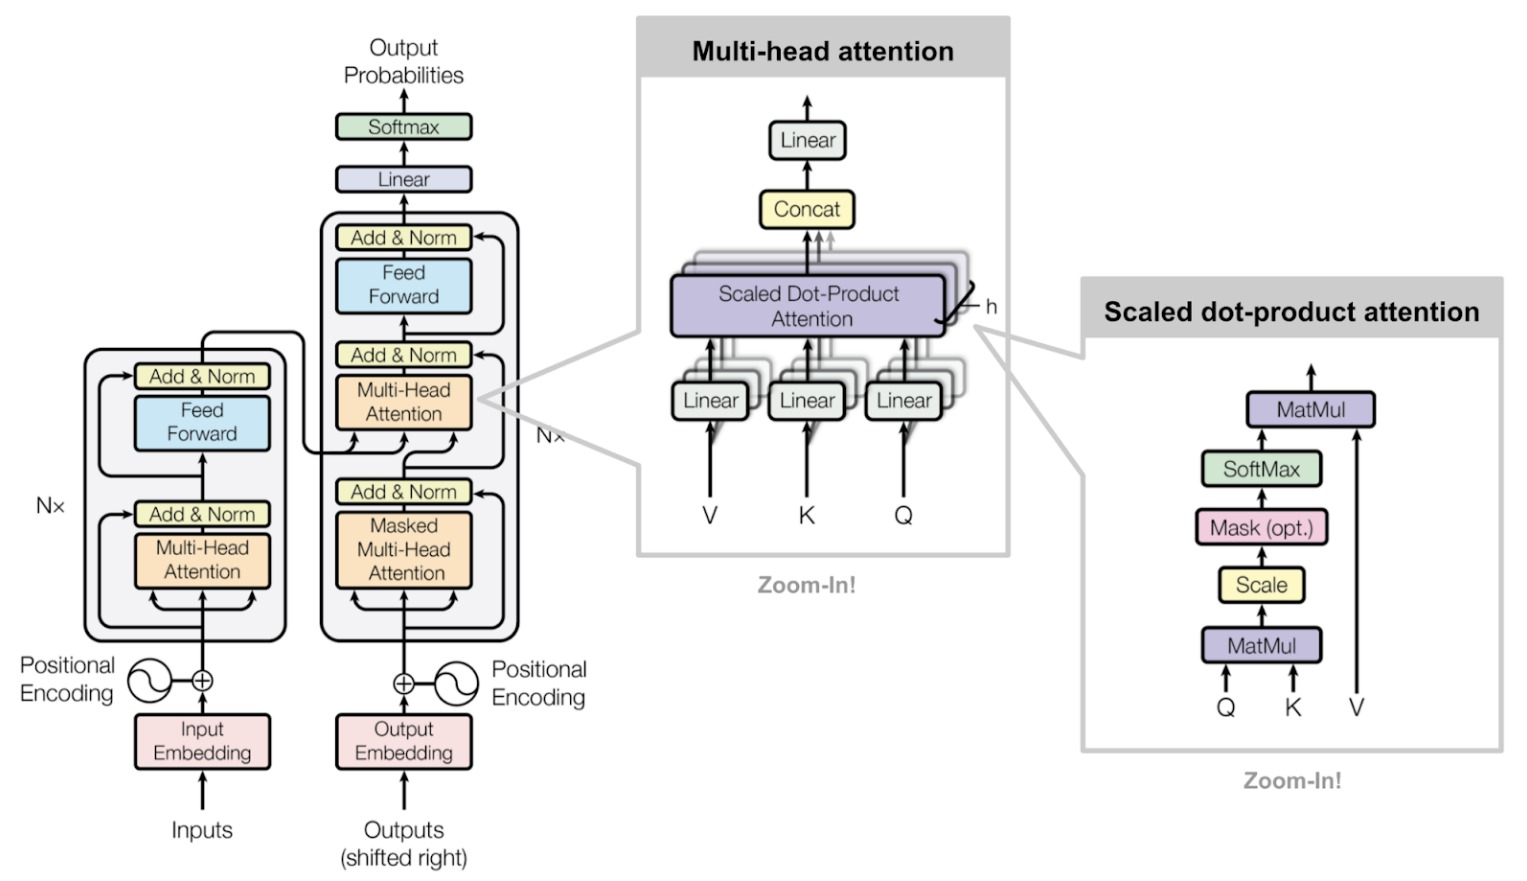
\includegraphics[width=0.6\textwidth]{WhatsApp Image 2024-05-29 at 14.31.19.jpeg}
    \caption{BERT Attention Mechanism}
    \label{fig:bert_attention}
\end{figure}

\section{Experimental Results}

\subsection{SVM Model Performance}
The SVM model is trained using TF-IDF and lemmatization features. The model is evaluated on the test set using metrics such as accuracy, precision, recall, and F1-score. The results are visualized in Figure \ref{fig:accuracy} and summarized in Table \ref{tab:classification_report}

\begin{table}[H]
    \centering
    \begin{tabular}{lcccc}
    \hline
    Class & Precision & Recall & F1-Score & Support \\
    \hline
    -1 & 0.74 & 0.86 & 0.80 & 159494 \\
    1 & 0.84 & 0.69 & 0.76 & 160506 \\
    \hline
    Accuracy & \multicolumn{4}{c}{0.77931875} \\
    Macro Avg & 0.79 & 0.78 & 0.78 & 320000 \\
    Weighted Avg & 0.79 & 0.78 & 0.78 & 320000 \\
    \hline
    \end{tabular}
    \caption{Classification Report for SVM Model}
    \label{tab:classification_report}
    \end{table}

\begin{figure}[H]
    \centering
    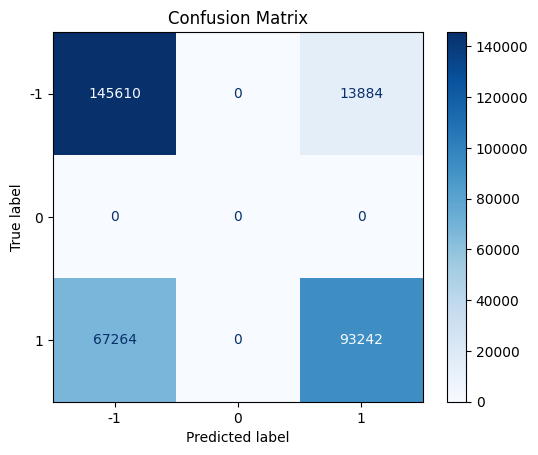
\includegraphics[width=0.6\textwidth]{svm_50epoch_tfidf.png}
    \caption{Confusion Matrix for SVM Model}
    \label{fig:accuracy}
\end{figure}

\subsection{CNN Model Performance}
The CNN model is trained using only tokenization and lemmatization features. The model's performance is evaluated on the test set, and the results are visualized in the following figures.

\begin{figure}[H]
    \centering
    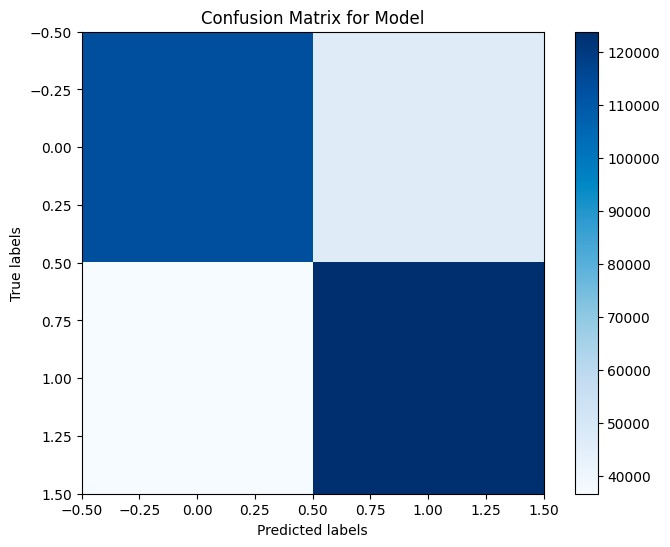
\includegraphics[width=0.6\textwidth]{WhatsApp Image 2024-05-29 at 02.36.54 (1).jpeg}
    \caption{Confusion Matrix for CNN Model}
    \label{fig:cnn_confusion_matrix}
\end{figure}

\begin{figure}[H]
    \centering
    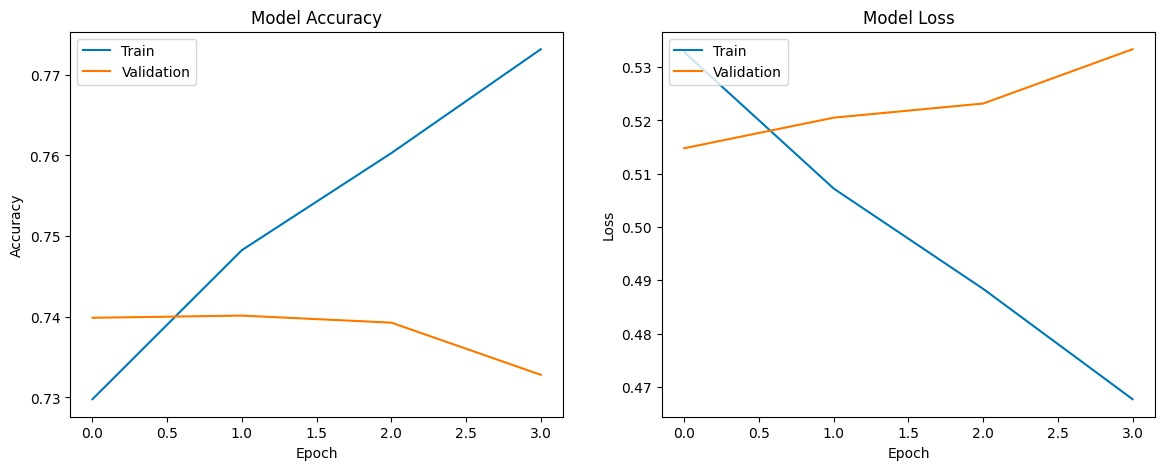
\includegraphics[width=0.8\textwidth]{WhatsApp Image 2024-05-29 at 02.37.14.jpeg}
    \caption{Training and Validation Accuracy/Loss for CNN Model}
    \label{fig:cnn_training_validation}
\end{figure}

\begin{table}[H]
    \centering
    \begin{tabular}{lcccc}
    \hline
    Class & Precision & Recall & F1-Score & Support \\
    \hline
    0 & 0.76 & 0.71 & 0.73 & 159494 \\
    1 & 0.73 & 0.77 & 0.75 & 160506 \\
    \hline
    Accuracy & \multicolumn{4}{c}{0.740409375} \\
    Macro Avg & 0.74 & 0.74 & 0.74 & 320000 \\
    Weighted Avg & 0.74 & 0.74 & 0.74 & 320000 \\
    \hline
    \end{tabular}
    \caption{Classification Report for CNN Model}
    \label{tab:cnn_classification_report}
\end{table}

\subsection{CNN Model Performance with GloVe Embeddings}
The CNN model incorporating GloVe embeddings was trained to enhance the representation of the text data. The model's performance was evaluated on the test set, and the results are summarized below.

\begin{figure}[H]
    \centering
    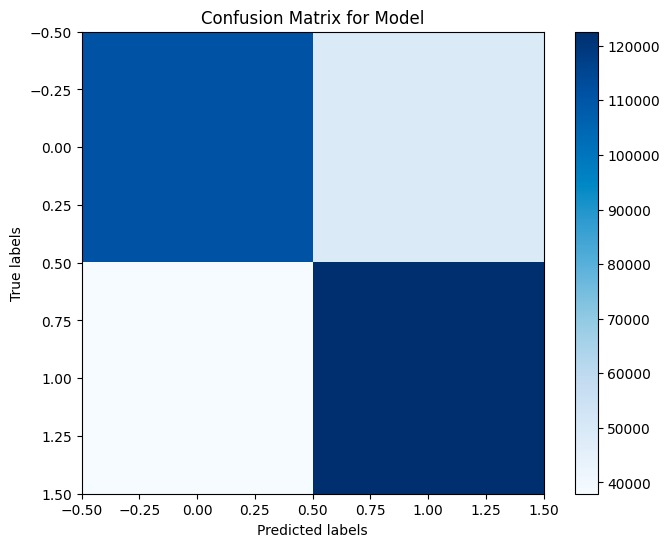
\includegraphics[width=0.6\textwidth]{WhatsApp Image 2024-05-29 at 02.38.06 (1).jpeg}
    \caption{Confusion Matrix for CNN Model with GloVe Embeddings}
    \label{fig:cnn_glove_confusion_matrix}
\end{figure}

\begin{figure}[H]
    \centering
    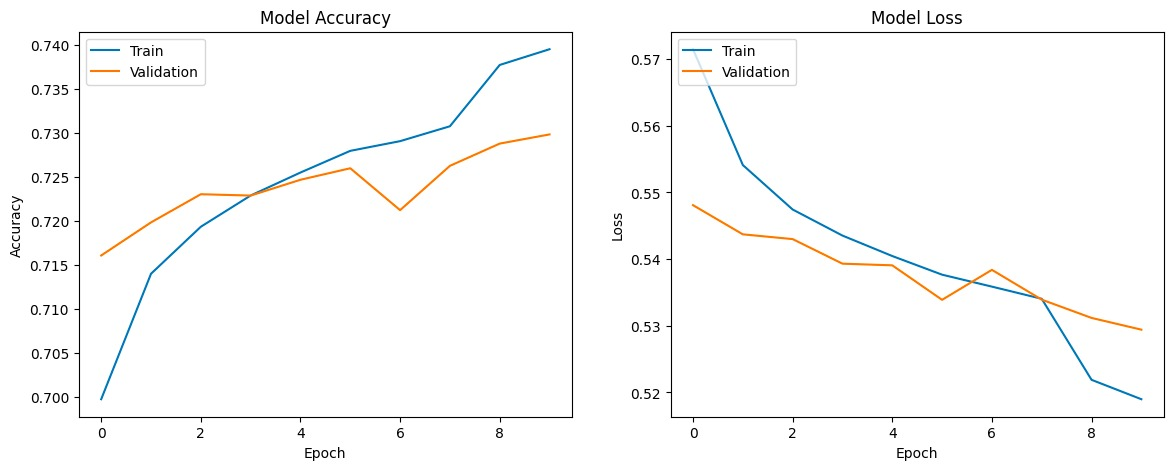
\includegraphics[width=0.8\textwidth]{WhatsApp Image 2024-05-29 at 02.38.06.jpeg}
    \caption{Training and Validation Accuracy/Loss for CNN Model with GloVe Embeddings}
    \label{fig:cnn_glove_training_validation}
\end{figure}

\begin{table}[H]
    \centering
    \begin{tabular}{lcccc}
    \hline
    Class & Precision & Recall & F1-Score & Support \\
    \hline
    0 & 0.74 & 0.69 & 0.72 & 159494 \\
    1 & 0.72 & 0.76 & 0.74 & 160506 \\
    \hline
    Accuracy & \multicolumn{4}{c}{0.7293} \\
    Macro Avg & 0.73 & 0.73 & 0.73 & 320000 \\
    Weighted Avg & 0.73 & 0.73 & 0.73 & 320000 \\
    \hline
    \end{tabular}
    \caption{Classification Report for CNN Model with GloVe Embeddings}
    \label{tab:cnn_glove_classification_report}
\end{table}

The CNN model with GloVe embeddings achieved an accuracy of 72.93\% on the test set. The confusion matrix (Figure \ref{fig:cnn_glove_confusion_matrix}) provides a visual representation of the true and predicted labels, indicating the model's performance in distinguishing between positive and negative sentiments. The training and validation accuracy/loss curves (Figure \ref{fig:cnn_glove_training_validation}) show the model's learning progression over epochs. The classification report (Table \ref{tab:cnn_glove_classification_report}) summarizes the precision, recall, F1-score, and support for each class, highlighting the model's effectiveness in sentiment classification tasks.


\subsection{BERT Model Performance}
The BERT model was trained on a subset of 15,000 tweets from the Sentiment140 dataset. This model leverages the transformer architecture to capture contextual information from both directions in the text, which is particularly effective for sentiment analysis. The performance of the BERT model on the test set is evaluated using precision, recall, F1-score, and support metrics.

The results are summarized as follows:

\begin{table}[H]
    \centering
    \begin{tabular}{lcccc}
    \hline
    Class & Precision & Recall & F1-Score & Support \\
    \hline
    Negative & 0.81 & 0.80 & 0.81 & 1476 \\
    Positive & 0.81 & 0.82 & 0.81 & 1524 \\
    \hline
    Accuracy & \multicolumn{4}{c}{0.81} \\
    Macro Avg & 0.81 & 0.81 & 0.81 & 3000 \\
    Weighted Avg & 0.81 & 0.81 & 0.81 & 3000 \\
    \hline
    \end{tabular}
    \caption{Classification Report for BERT Model}
    \label{tab:bert_classification_report}
\end{table}

\begin{figure}[H]
    \centering
    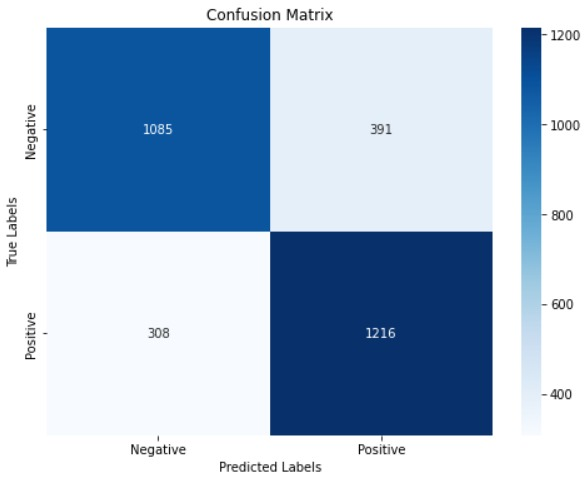
\includegraphics[width=0.6\textwidth]{xyz.png}
    \caption{Confusion Matrix for BERT Model}
    \label{fig:bert_confusion_matrix}
\end{figure}

The confusion matrix for the BERT model, as shown in Figure \ref{fig:bert_confusion_matrix}, provides a visual representation of the true and predicted labels, indicating the model's performance in distinguishing between positive and negative sentiments.

Additionally, we performed an analysis using a pre-trained BERT model available from Hugging Face, specifically the \texttt{MarieAngeA13/Sentiment-Analysis-BERT}. The performance metrics for this pre-trained model are as follows:

\begin{table}[H]
    \centering
    \begin{tabular}{lcccc}
    \hline
    Class & Precision & Recall & F1-Score & Support \\
    \hline
    Negative & 0.78 & 0.74 & 0.76 & 1476 \\
    Positive & 0.76 & 0.80 & 0.78 & 1524 \\
    \hline
    Accuracy & \multicolumn{4}{c}{0.77} \\
    Macro Avg & 0.77 & 0.77 & 0.77 & 3000 \\
    Weighted Avg & 0.77 & 0.77 & 0.77 & 3000 \\
    \hline
    \end{tabular}
    \caption{Classification Report for Pre-trained BERT Model}
    \label{tab:pretrained_bert_classification_report}
\end{table}

The pre-trained model demonstrates slightly lower performance compared to our custom-trained BERT model, but still shows strong results, highlighting the effectiveness of transfer learning for sentiment analysis tasks.
\section{Conclusion}
This study compared the performance of three different types of models for tweet sentiment analysis: Support Vector Machine (SVM), Convolutional Neural Networks (CNN) combined with Recurrent Neural Networks (RNN), and Bidirectional Encoder Representations from Transformers (BERT). Each model represents a distinct stage in the evolution of machine learning techniques, offering unique strengths and weaknesses in handling sentiment analysis tasks.

The SVM model, combined with TF-IDF and GloVe embeddings, demonstrated effective performance in classifying tweet sentiments. The model achieved an accuracy of 77.93\%, with balanced precision, recall, and F1-scores for both positive and negative sentiment classes. SVMs are particularly adept at handling high-dimensional feature spaces typical of text data, and their performance in this study underscores their continued relevance for sentiment analysis tasks. However, the SVM model may struggle to capture complex patterns and contextual nuances that more advanced models can detect. Future work with SVM could involve exploring more sophisticated feature extraction techniques and hyperparameter tuning to further improve its performance.

The CNN models in this study showed that while tokenization and lemmatization-based feature extraction can yield strong results, the integration of GloVe embeddings did not provide the anticipated performance boost. The simpler CNN model, which relied solely on tokenization and lemmatization, achieved a marginally better accuracy of 74\% compared to the 73\% accuracy of the GloVe-embedded model. This discrepancy suggests that the parameters of the GloVe embeddings might not have been optimally tuned for this specific task. Additionally, the longer training times for the GloVe model indicate challenges in efficiently fitting the data within the provided epochs. Despite these findings, CNNs remain valuable due to their ability to capture local patterns and their computational efficiency. Future research could focus on optimizing embedding parameters or exploring other advanced embeddings to enhance CNN performance.

The RNN model, specifically the Bidirectional LSTM (BiLSTM) architecture, outperformed both CNN models, achieving an accuracy of 78\%. The BiLSTM's ability to capture long-term dependencies and contextual information from both past and future tokens contributed to its superior performance. This model effectively differentiated between positive and negative sentiments, leading to higher true positive and true negative counts and reducing misclassifications. However, the complexity of the LSTM layers resulted in significantly slower training times compared to CNNs. The trade-off between accuracy and computational efficiency is a critical consideration, and future work could explore ways to optimize LSTM training or combine RNNs with other techniques to balance performance and efficiency.

The BERT model demonstrated the highest performance among the models tested, with an accuracy of 81\%. Both the custom-trained and pre-trained BERT models showcased BERT's ability to understand and process contextual information from tweets, capturing nuances that simpler models might miss. The advanced attention mechanisms and bidirectional context understanding of BERT provide significant advantages in sentiment analysis applications. Future work could involve fine-tuning BERT with additional data, experimenting with different pre-trained versions, and exploring hybrid approaches that combine traditional and deep learning models to further enhance sentiment analysis solutions.

In conclusion, each model type offers unique advantages for tweet sentiment analysis. SVMs provide robust performance with simpler feature extraction techniques, CNNs offer computational efficiency and strong local pattern recognition, RNNs excel in capturing long-term dependencies, and BERT leads in overall performance due to its advanced contextual understanding. Future research should focus on optimizing these models and exploring hybrid approaches to leverage their strengths and mitigate their weaknesses, ultimately advancing the field of sentiment analysis.


\end{document}
